\section{Determine the strength of a poker hand}
\label{sec:part1}
Our first step towards developing the APA is to find a way to determine the strength of any given hand in any game state. In this chapter we will answer the following problem statement: 

\vspace{4mm}
\begin{statementBox2}{Problem statement 1}
How can APA determine the strength of a poker hand in any game state?
\end{statementBox2}
\vspace{4mm}

The strength of a hand reflects the probability of winning therefore the stronger a hand is the more likely one are to win. Since the player does not know the outcome of the community cards during a round of poker, the player has to calculate the probability of winning based on the possible outcomes of the community cards. It is too time consuming to check every outcome as there are more than 250 millions different outcomes of community cards alone. In order to find the probability of winning without having to check all possible outcomes, one can instead make an estimate rather than calculating the true probability. 

\subsection{Design}
When trying to estimate the strength of a hand, two options exist.

The first option is to create a simplified formula. Such formulas already exist, but since they are very simple they tend to be rather inaccurate. This option is straight forward, but the disadvantage is, that it is hard to make a formula that is accurate for every game state.

The second option is to use the Monte Carlo method to simulate a large amount of games and get the distribution of outcomes. This distribution can then be used to find the probability of winning.

For a human player a simplified formula is necessary but due to the computational power of a computer the Monte Carlo method is optimal for the APA. A computer can perform thousands of simulations in no time. This method also gives a trade-off between accuracy and the number of simulations. This allows us to adjust the accuracy of the probability by adjusting the number of simulations. The major poker sites also use the Monte Carlo method to determine each players probability of winning.

The solution is implemented as a subsystem that uses the Monte Carlo method. We will refer to this subsystem as the calculator.

\RestyleAlgo{boxruled}
\LinesNumbered
\vspace{4mm}
\begin{algorithm}[H]
  \KwData{Hole cards, number of opponents, community cards (optional)}
  \KwResult{win = 1, draw = 0, lose = -1}
Random missing community cards\;
Determine rank of players hand\;
  \ForEach{opponent} {
    Determine rank of opponents hand\;
    \If{opponent has stronger hand}{\Return ~-1\;}
    \ElseIf{opponent has same hand}{\Return 0\;}
  }
  \Return 1\;
\caption{Pseudo-code for a single simulation}
\end{algorithm}
\vspace{4mm}

The calculator takes three arguments: the hole cards of the player, the number of opponents, and the community cards (optional). The calculator simulates a pre-defined number of rounds and returns an object containing the distribution of wins, draws, and loses.

The calculator considers it a win only if the hand beats every other hand of the opponents.

Algorithm 1 shows the pseudo-code for determining the result of a single simulation.

In order to ensure the quality of the calculator, we have the following requirements:
\begin{itemize}
\item It must have a maximum error percentage of one percent. (deviation from the true probability)
\item It must calculate the probability in less than five seconds.
\item It must be able to return the probability of winning with a given hand in any game state with up to ten players.
\end{itemize}

\subsubsection{Monte Carlo method}
The Monte Carlo method is used to find the distribution of outcomes for a domain. Given a set of user defined inputs the Monte Carlo method performs the simulation to find the outcome. For each simulation the method tracks the outcomes and as the number of simulations increases, so will the accuracy of the distribution. This distribution can help to get a better understanding of the examined domain.

\subsection{Test}
We have created tests to ensure the calculator fulfils all the requirements. 
 
In order to find the accuracy of the probabilities we first need to know the true probabilities. For this we use caniwin \cite{caniwin}. Caniwin is a website that has simulated all possible outcomes of any pre-flop hands. Caniwin's results are limited to the pre-flop game state, so we can only test the calculator for this game state.

The number of simulations affects the error percentage as well as the calculation time. We start by finding a number of simulations that meets the first and second requirement. We test what number of simulations are needed in order to get a maximum error of one percent. Afterwards we will find the number of simulations that results in a calculation time in less than five seconds.

Once we have a suitable number of simulations we test if the calculator finds the correct probability using this number of simulations.

\subsubsection{Finding the maximum error}
\label{sec:mc-test1}
As mentioned earlier the number of simulations affects the accuracy of the result. In this test we will find the number of simulations that fulfils the requirement of having a maximum error percentage of one percent.

Each test is performed with the hand J\clubsuit ~ J\diamondsuit ~ in pre-flop with one opponent. The calculator calculates the probability 50 times for each test. The true probability found by caniwin is $\sim$77,1~\%. 
We then calculate the error of each calculation using the formula:

\[err = P_{O} - P_{T}\]

Here $P_{O}$ is the probability found by the calculator and $P_{T} $ is the true probability. 

We inserted the results of each test in a graph, see figure \ref{fig:mc1}, \ref{fig:mc10}, and \ref{fig:mc50}. 
Each test result is indicated with a red dot. The three graphs clearly shows that when using a higher amount of simulations, the more accurate the probability are.

Table \ref{tab:mc-total} shows the range of results as well as the maximum error for the tests. From this we can see that 50.000 simulations fulfils our first requirements.

\begin{figure}[H]
  \center
    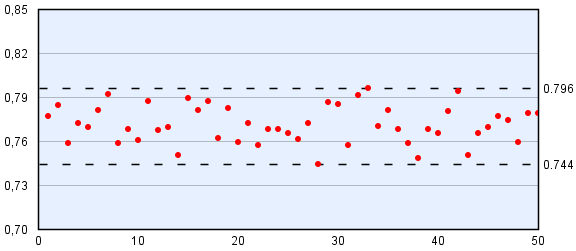
\includegraphics[scale=0.775]{images/MonteCarlo/1k.png}
  \caption{Result of the calculator with 1000 simulations \label{fig:mc1}}
\end{figure}

\begin{figure}[H]
  \center
    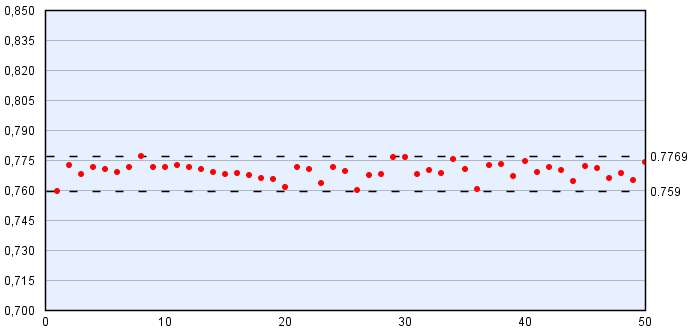
\includegraphics[scale=0.775]{images/MonteCarlo/10k.png}
  \caption{Result of the calculator with 10.000 simulations \label{fig:mc10}}
\end{figure}

\begin{figure}[H]
  \center
    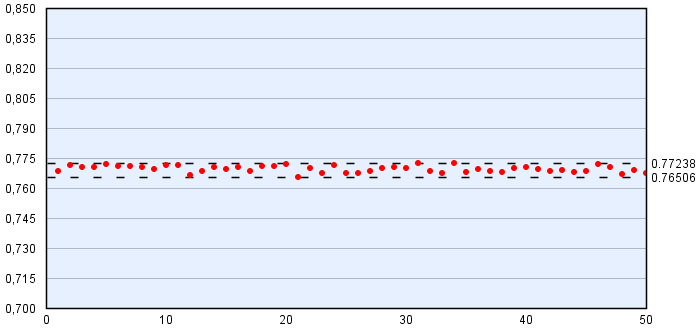
\includegraphics[scale=0.775]{images/MonteCarlo/50k.png}
  \caption{Result of the calculator with 50.000 simulations \label{fig:mc50}}
\end{figure}

\begin{table}[H]
  \center
  \begin{tabular}{ | l | l | l | }
    \hline
    simulations & range (\%) & max error (\%) \\
    \hline                       
    1000 & 5,2 & 2,7 \\
    10.000 & 2,2 & 1,5 \\
    50.000 & 0,9 & 0,7 \\
  \hline  
  \end{tabular}
  \caption{Combined test results from running the calculator with different numbers of simulations. \label{tab:mc-total}}
\end{table}
\vspace{4mm}

\subsubsection{Finding the calculation time}
In this test we run the calculator 100 times with the same hand in order to find an average computation time. 
In table \ref{tab:mc-time} the average computation time can be seen. As we expect the computation time increases as the number of simulations increases. 

\vspace{4mm}
\begin{table}[H]
  \center
  \begin{tabular}{ | l | l | }
    \hline
    simulations & Average computation time\\
    \hline                       
    1000 & $\sim$0,01 seconds\\
    10.000 & $\sim$0,04 seconds\\
    50.000 & $\sim$0,15 seconds\\
  \hline  
  \end{tabular}
  \caption{Calculation times from running the calculator with different numbers of simulations. \label{tab:mc-time}}
\end{table}
\vspace{4mm}

Luckily, using 50.000 simulations gives an average computation time of $\sim$0,15 seconds which also satisfies the second requirement. We therefore settle for 50.000 simulation as the number of simulations for the calculator.

\subsubsection{Determining the correctness of the calculator}
To test if the calculator can calculate the correct probabilities, we find the probability of a number of different pre-flop hands and compare the result with the true probability. Every test is preformed with 50.000 simulations against one opponent. We use the formula described in section \ref{sec:mc-test1}:
\[err = P_{O} - P_{T}\]

The result can be seen in table \ref{tab:pre-flop-test}. From the results we can see that for all tests the error percentage is less than one percent and the calculator therefore works for the pre-flop.
\vspace{4mm}
\def\arraystretch{1.5}
\begin{table}[H]
  \center
  \begin{tabular}{ | l | l | l | l | }
  	\hline
  	hole cards & $P_{O}$ (\%) & $P_{T}$ (\%) & error (\%) \\
  	\hline                       
    A\clubsuit ~ A\diamondsuit & 85,2 & 84,9 & 0,3 \\
    8\clubsuit ~ 8\diamondsuit & 67,9 & 68,7 & 0,8 \\
    Q\clubsuit ~ k\clubsuit & 62,8 & 62,4 & 0,4 \\
    A\heartsuit ~ 8\spadesuit & 58,8 & 60,5 & 0,7 \\
    J\spadesuit ~ Q\diamondsuit & 57,2 & 56,9 & 0,3 \\
    10\heartsuit ~ J\heartsuit & 56,7 & 56,2 & 0,5 \\
    3\diamondsuit ~ 3\spadesuit & 53,0 & 52,8 & 0,2 \\
    2\diamondsuit ~ 2\heartsuit & 49,5 & 49,4 & 0,1 \\
    9\diamondsuit ~ 3\spadesuit & 37,8 & 37,4 & 0,4 \\
    2\diamondsuit ~ 7\diamondsuit & 35,5 & 35,4 & 0,1 \\
    2\diamondsuit ~ 7\heartsuit & 31,9 & 31,7 & 0,2 \\
  	\hline   	
  \end{tabular}
  \caption{Test results for different hole cards in pre-flop with one opponent. \label{tab:pre-flop-test}}
\end{table}
\vspace{4mm} 

Testing the calculator for other game states is a bit problematic because we were not able to find any probabilities for anything but pre-flop. Instead we calculate the probability of some hands during all game states. 

In table \ref{tab:percent} we can see the results. For the first situation (A\clubsuit ~ K\diamondsuit) the player start with a strong hand but does not hit anything from the community cards. As expected the probability decreases. The second hand (2\diamondsuit ~ 5\spadesuit) is weak until the turn where it hits a straight. This is also clearly shown by the percentages. Likewise the third hand (8\spadesuit ~ 9\spadesuit) hits a flush on the river and the probability increases drastically. Finally we have the hand (5\spadesuit ~ 5\clubsuit) where there is a straight from the community cards. This results in a zero percent win chance because the community cards are public and therefore the result is either a draw or a lose.
The data suggests that the calculator works for all game states.
\vspace{4mm}
\def\arraystretch{1.5}
\begin{table}[H]
  \center
  \begin{tabular}{ | l | l | l | l | l | l | }
  	\hline
  	hole cards & community cards & pre-flop (\%) & flop (\%) & turn (\%) & river (\%) \\
  	\hline 
  	A\clubsuit ~ K\diamondsuit & 3\spadesuit ~ 7\clubsuit ~ T\clubsuit ~ 8\diamondsuit ~ 2\spadesuit & 64,5 & 54,4 & 41,7 & 35,6\\
  	\hline                     
    2\diamondsuit ~ 5\spadesuit & 3\spadesuit ~ 6\diamondsuit ~ K\diamondsuit ~ 4\heartsuit ~ 7\spadesuit & 29,7 & 28,2 & 92,8 & 94,2 \\
    \hline
    8\spadesuit ~ 9\spadesuit & 2\diamondsuit ~ K\spadesuit ~ 3\spadesuit ~ A\clubsuit ~ T\spadesuit & 49,1 & 53,5 & 38,5 & 99,7 \\    
    \hline
    5\spadesuit ~ 5\clubsuit & A\diamondsuit ~ K\heartsuit ~ Q\spadesuit ~ J\diamondsuit ~ T\heartsuit & 58,5 & 48,0 & 34,4 & 0,0 \\    
  	\hline   	
  \end{tabular}
    \caption{Test results for different hole cards in pre-flop, flop, turn, and river with one opponent \label{tab:percent}}
\end{table}
\vspace{4mm} 

\begin{table}[H]
  \center
  \begin{tabular}{ | l | l | l | l | l | l | l | l | l | l |}
  	\hline
  	opponents & 1 & 2 & 3 & 4 & 5 & 6 & 7 & 8 & 9 \\
  	\hline 
  	win probability (\%) & 85,2 & 73,4 & 64,0 & 56,1 & 49,5 & 43,9 & 39,1 & 35,0 & 31,6 \\
  	\hline                       	
  \end{tabular}
    \caption{Chance of winning with the hole cards A\spadesuit ~ A\clubsuit ~ in pre-flop \label{tab:winchance}}
\end{table}

From table \ref{tab:winchance} we can see that the probability also decreases as the number of players increases, which suggest it works for multiple players as well.

The calculator passed all tests and seems to work in every situation. 

\subsection{Discussion}
For the implementation of the calculator the Monte Carlo method was exactly what was needed to fulfil the needs. The calculator can calculate the probability with an error percentage of less than one percent when using 50.000 simulations. This solution can be used for any poker state with up to ten players.	

Since we compare the results of the calculator to caniwin, we need to ensure the reliability of that source. Bobby, the author of caniwin, has a bachelor in math from the University of Southern California in LA. The rest of the thesis is written on the assumption that the results from caniwin is correct

Alternatively we could have created our own formula to calculate a rank, or used an existing one, for instance the Chen formula. However, this has been beyond the scope of this thesis.

\subsection{Conclusion}
In this chapter we have answered the question:
\vspace{4mm}
\begin{statementBox2}{Problem statement 1}
How can APA determine the strength of a poker hand in any game state?
\end{statementBox2}
\vspace{4mm}

We define the strength of a poker hand as the probability of winning with that hand.

We have implemented a subsystem called the calculator that can estimate the probability of winning with any given set of hole cards. The calculator uses the Monte Carlo method and it works for every poker state with up to ten players. 50.000 simulations  met the requirements we made for the calculator.   

The calculator has a maximal error percentage of one percent compared to the true probability and performs the calculation in $\sim$0,15 seconds.
